\section{Comentario}
\label{sec:comentario}
De vez en cuando, no solamente el código generado va a necesitar una breve
explicación acerca de cual es su función, sino que puede llegar a ser el caso
que el modelo en sí también necesite una explicación sobre alguna parte en
especial, para que los involucrados con el modelo puedan saber de que se trata.
El lenguaje propuesto permite este comportamiento mediante la inclusión, no
solamente de un mecanismo que permita comentar el código resultante, sino que
tambien se puede comentar partes del modelo que no se deben tener en cuenta.

\subsection{Comentarios Director}
\label{sub:comentariosdrt}
Aqui se detallan las reglas a seguir para poder realizar un comentario en el
modelo, es decir, este comentario no sería tomado en cuenta a la hora de
parsear el archivo para poder obtener el código.

Dentro del área de los comentarios, en el lenguaje se ofrece, al igual que gran
parte de los lenguajes de propósito general, la posibilidad de introducir
comentarios de línea y comentarios multilínea.

La expresión para el BNF de un comentario tanto de línea como uno multilínea
está dada de la siguiente manera:

\begin{lstlisting} [language=Java, basicstyle=\footnotesize\ttfamily,
caption={BNF - Comentario de línea}]
	<comentario-linea> ::= "##" <texto>
\end{lstlisting}

\begin{figure}[H]
	\centering
	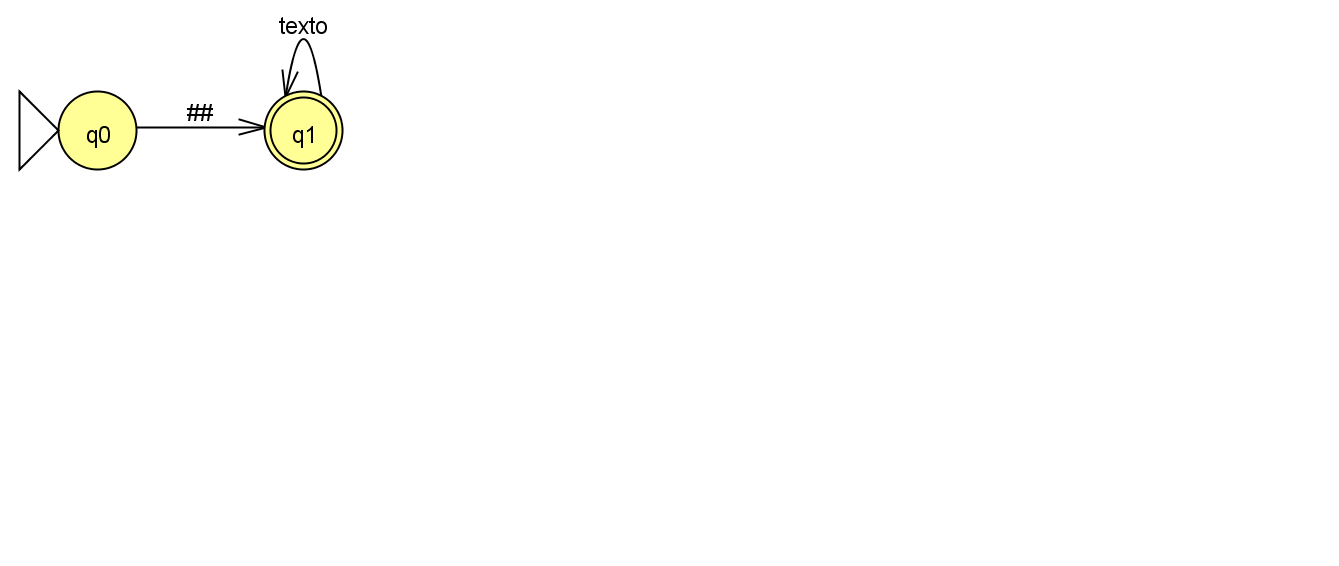
\includegraphics[width=.7\linewidth]{automatas_finitos/comentarioDrtLinea.png}
	\caption{Autómata finito - Comentario de línea}
	\label{fig:af_com_linea}
\end{figure}

\begin{lstlisting} [language=Java, basicstyle=\footnotesize\ttfamily,
caption={BNF - Comentario multilínea}]
	<comentario-multilinea> ::= "#{" <texto> "}#"
\end{lstlisting}

\begin{figure}[H]
	\centering
	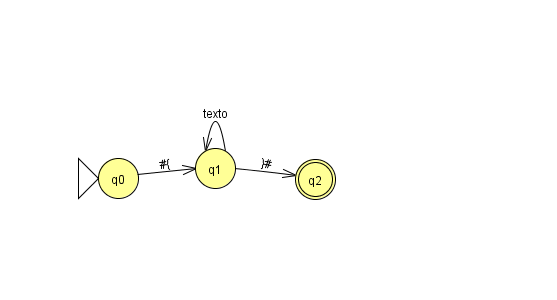
\includegraphics[width=.7\linewidth]{automatas_finitos/comentarioDrtMultilinea.png}
	\caption{Autómata finito - Comentario multilínea}
	\label{fig:af_com_multi}
\end{figure}

Las respectivas expresiones regulares para ambos tipos de comentarios se
describen a continuación:

\begin{lstlisting} [caption={Regex - Comentario de Línea}, language=java, basicstyle=\footnotesize\ttfamily]
	regex: /##[a-za-z0-9 \n\r\t]*/
\end{lstlisting}

\begin{lstlisting} [caption={Regex - Comentario Multilínea}, language=java, basicstyle=\footnotesize\ttfamily]
	regex: /#{[a-za-z0-9 \n\r\t]}#*/
\end{lstlisting}

\subsection{Comentarios para Lenguaje}
\label{sub:comentarioleng}
Estos comentarios se tendrán en cuenta a la hora de parsear el documento esto
se debe a que serán contenidos por el código resultante. Es decir, son un
comentario para el codigo que resulte del módelo que se tenga en cuestión.

Nuevamente, aquí se tiene la posibilidad de establecer los comentarios de línea
y comentarios multilínea,

\begin{lstlisting} [language=Java, basicstyle=\footnotesize\ttfamily,
caption={BNF - Comentario de línea (lenguaje)}]
	<comentario-linea> ::= "//" <texto>
\end{lstlisting}

\begin{figure}[H]
	\centering
	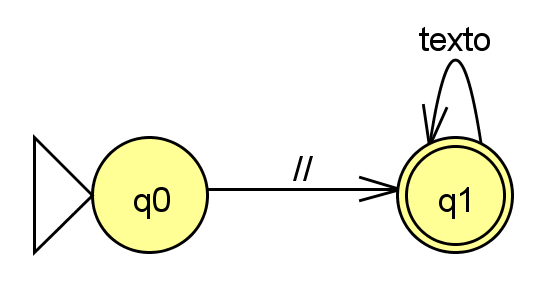
\includegraphics[width=.7\linewidth]{automatas_finitos/comentarioLengLinea.png}
	\caption{Autómata finito - Comentario de línea (lenguaje)}
	\label{fig:af_com_linea_leng}
\end{figure}

\begin{lstlisting} [language=Java, basicstyle=\footnotesize\ttfamily,
caption={BNF - Comentario multilínea (lenguaje)}]
	<comentario-multilinea> ::= "/*" <texto> "*/"
\end{lstlisting}

\begin{figure}[H]
	\centering
	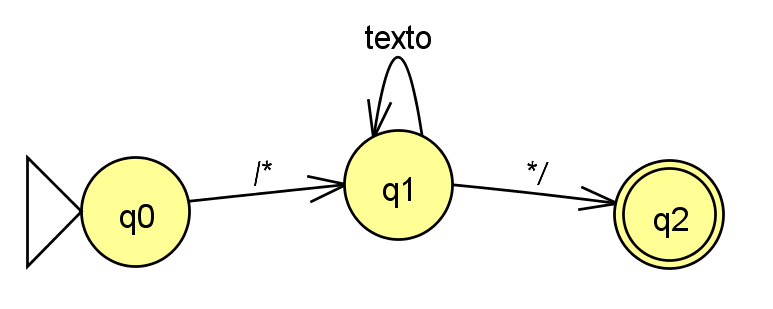
\includegraphics[width=.7\linewidth]{automatas_finitos/comentarioLengMultilinea.png}
	\caption{Autómata finito - Comentario multilínea (lenguaje)}
	\label{fig:af_com_multi_leng}
\end{figure}

Las respectivas expresiones regulares para ambos tipos de comentarios se
describen a continuación:

\begin{lstlisting} [language=java, basicstyle=\footnotesize\ttfamily,
caption={Regex - Comentario de línea (lenguaje)}]
	regex: /\/\/[a-za-z0-9 \n\r\t]*/
\end{lstlisting}

\begin{lstlisting} [language=java, basicstyle=\footnotesize\ttfamily,
caption={Regex - Comentario multilínea (lenguaje)}]
	regex: /\/\*[a-za-z0-9 \n\r\t]*\*\//
\end{lstlisting}

